\documentclass{article}\usepackage[]{graphicx}\usepackage[]{color}
%% maxwidth is the original width if it is less than linewidth
%% otherwise use linewidth (to make sure the graphics do not exceed the margin)
\makeatletter
\def\maxwidth{ %
  \ifdim\Gin@nat@width>\linewidth
    \linewidth
  \else
    \Gin@nat@width
  \fi
}
\makeatother

\definecolor{fgcolor}{rgb}{0.345, 0.345, 0.345}
\newcommand{\hlnum}[1]{\textcolor[rgb]{0.686,0.059,0.569}{#1}}%
\newcommand{\hlstr}[1]{\textcolor[rgb]{0.192,0.494,0.8}{#1}}%
\newcommand{\hlcom}[1]{\textcolor[rgb]{0.678,0.584,0.686}{\textit{#1}}}%
\newcommand{\hlopt}[1]{\textcolor[rgb]{0,0,0}{#1}}%
\newcommand{\hlstd}[1]{\textcolor[rgb]{0.345,0.345,0.345}{#1}}%
\newcommand{\hlkwa}[1]{\textcolor[rgb]{0.161,0.373,0.58}{\textbf{#1}}}%
\newcommand{\hlkwb}[1]{\textcolor[rgb]{0.69,0.353,0.396}{#1}}%
\newcommand{\hlkwc}[1]{\textcolor[rgb]{0.333,0.667,0.333}{#1}}%
\newcommand{\hlkwd}[1]{\textcolor[rgb]{0.737,0.353,0.396}{\textbf{#1}}}%

\usepackage{framed}
\makeatletter
\newenvironment{kframe}{%
 \def\at@end@of@kframe{}%
 \ifinner\ifhmode%
  \def\at@end@of@kframe{\end{minipage}}%
  \begin{minipage}{\columnwidth}%
 \fi\fi%
 \def\FrameCommand##1{\hskip\@totalleftmargin \hskip-\fboxsep
 \colorbox{shadecolor}{##1}\hskip-\fboxsep
     % There is no \\@totalrightmargin, so:
     \hskip-\linewidth \hskip-\@totalleftmargin \hskip\columnwidth}%
 \MakeFramed {\advance\hsize-\width
   \@totalleftmargin\z@ \linewidth\hsize
   \@setminipage}}%
 {\par\unskip\endMakeFramed%
 \at@end@of@kframe}
\makeatother

\definecolor{shadecolor}{rgb}{.97, .97, .97}
\definecolor{messagecolor}{rgb}{0, 0, 0}
\definecolor{warningcolor}{rgb}{1, 0, 1}
\definecolor{errorcolor}{rgb}{1, 0, 0}
\newenvironment{knitrout}{}{} % an empty environment to be redefined in TeX

\usepackage{alltt}
\usepackage[utf8]{inputenc}
\usepackage{amsmath}
\usepackage{graphicx}
%\usepackage{bbold}
\usepackage{tikz}
%\usepackage{silence}
\usepackage{mdframed}
%\WarningFilter{mdframed}{You got a bad break}
\usepackage[colorinlistoftodos]{todonotes}
%\usepackage{listings}
\usepackage{listingsutf8}
\usepackage{color}
\colorlet{exampcol}{blue!10}
\usepackage{multicol}
\usepackage[answerdelayed]{exercise}
\usepackage{booktabs}
\usepackage{caption}

\title{BIO311: Population Ecology\\ \textit{Prac 9: Population Matrices \& LTRE}}

\setcounter{tocdepth}{1} % Determines the depth of the table of contents;; 0:chapters, 1: chapters and sections, 2: chapters,sections and subsections

%\renewcommand{\theExercise}{\thechapter.\arabic{Exercise}}%
\IfFileExists{upquote.sty}{\usepackage{upquote}}{}
\begin{document}

\author{Timoth\'ee Bonnet \&\footnote{This document was co-authored by Tina Cornioley}\; Koen van Benthem\\\\
\tt{timothee.bonnet@ieu.uzh.ch}\\ \tt{koen.vanbenthem@ieu.uzh.ch}}

\date{Spring 2016}





\maketitle
\tableofcontents
\vspace{3cm}
\newpage

\subsubsection{Reproductive values}\label{Newfrhere}
The reproductive value vector represents the contribution of each individual to present and future reproduction. In other words, it gives how much an individual in a given age class contributes to the population on the long-term, including offspring of its offspring. That is: if we have a population and its matrix at time $t=1$, what proportion of individuals at a much later time will be descendants of individuals in age class $1$ at time $t=1$ and how many from individuals in age class $2$ etc. Mathematically, the reproductive value vector is the left eigenvector of the population matrix.
\begin{equation}
\vec{v}A=\lambda \vec{v}
\end{equation}
Please note that this time the vector is on the left side instead of on the right side of the matrix. This is why this is called a left eigenvector. Multiplication with the vector on the left side of the matrix looks as follows in 2 dimensions:
\begin{equation}
\begin{pmatrix} v_1 & v_2 \end{pmatrix} \begin{pmatrix} a_{1,1} & a_{1,2}\\ a_{2,1} & a_{2,2} \end{pmatrix} = \begin{pmatrix} v_1 a_{1,1} + v_2 a_{2,1} & v_1 a_{1,2} + v_2 a_{2,2} \end{pmatrix}
\end{equation}
Again, we take the row from the first element (in this case the vector) and multiply its elements by the elements of the first column of the second element (in these case a matrix). Adding up these contributions gives us the value for the first entry of the final vector. Compare this to what you would get if the order of the matrix and the vector would be the other way around.

To get the left eigenvector of a matrix, we need to perform the eigen analysis on the transpose of the projection matrix. (The transpose of a matrix is the matrix we get by exchanging the rows and the columns of that matrix. For example for the matrix $\boldsymbol{B}=\begin{pmatrix}a & b\\ c & d\end{pmatrix}$, $\boldsymbol{B}^T$ is the transpose of matrix $\boldsymbol{B}$ and $\boldsymbol{B}^T=\begin{pmatrix}a & c\\ b & d\end{pmatrix}$). More visually: when you transpose a matrix, you mirror its elements in the diagonal of that matrix. \texttt{t()} is the \texttt{R} function that transposes a matrix. If you do not remember what the function \texttt{eigen} does, reread the subsection \textit{asymptotic rate of increase} or aks \texttt{R} (\texttt{?eigen}).

\begin{knitrout}
\definecolor{shadecolor}{rgb}{0.969, 0.969, 0.969}\color{fgcolor}\begin{kframe}
\begin{alltt}
\hlstd{At}\hlkwb{<-}\hlkwd{t}\hlstd{(A)}
\end{alltt}


{\ttfamily\noindent\bfseries\color{errorcolor}{\#\# Error in t(A): objet 'A' introuvable}}\begin{alltt}
\hlstd{eigens.At}\hlkwb{<-}\hlkwd{eigen}\hlstd{(At)}
\end{alltt}


{\ttfamily\noindent\bfseries\color{errorcolor}{\#\# Error in as.matrix(x): objet 'At' introuvable}}\begin{alltt}
\hlstd{eigens.At}
\end{alltt}


{\ttfamily\noindent\bfseries\color{errorcolor}{\#\# Error in eval(expr, envir, enclos): objet 'eigens.At' introuvable}}\end{kframe}
\end{knitrout}
We apply the same proceedure as for the right eigenvector to find the left eigenvector and the eigenvalue. Write the code to extract the eigenvalue and the left eigenvector. Do you notice anything about the eigenvalue? Check that the found dominant left eigenvector is indeed a left eigenvector of the matrix with the dominant eigenvalue as its eigenvalue.\\[1.5ex]
\begin{knitrout}
\definecolor{shadecolor}{rgb}{0.969, 0.969, 0.969}\color{fgcolor}\begin{kframe}


{\ttfamily\noindent\bfseries\color{errorcolor}{\#\# Error in which.max(eigens.At\$values): objet 'eigens.At' introuvable}}

{\ttfamily\noindent\bfseries\color{errorcolor}{\#\# Error in eval(expr, envir, enclos): objet 'eigens.At' introuvable}}

{\ttfamily\noindent\bfseries\color{errorcolor}{\#\# Error in eval(expr, envir, enclos): objet 'eigens.At' introuvable}}

{\ttfamily\noindent\bfseries\color{errorcolor}{\#\# Error in eval(expr, envir, enclos): objet 'v' introuvable}}

{\ttfamily\noindent\bfseries\color{errorcolor}{\#\# Error in eval(expr, envir, enclos): objet 'rv' introuvable}}\end{kframe}
\end{knitrout}
\begin{mdframed}
\textbf{Additional information: Reproductive values more in depth}\\
If you want to understand the interpretation of the reproductive values more closely, take a look at the following (not too elegant) code:
\begin{knitrout}
\definecolor{shadecolor}{rgb}{0.969, 0.969, 0.969}\color{fgcolor}\begin{kframe}
\begin{alltt}
\hlstd{B}\hlkwb{<-}\hlkwd{matrix}\hlstd{(}\hlnum{4}\hlopt{*}\hlkwd{runif}\hlstd{(}\hlnum{9}\hlstd{),}\hlkwc{nrow}\hlstd{=}\hlnum{3}\hlstd{)} \hlcom{# We generate a random matrix}

\hlstd{B}
\end{alltt}
\begin{verbatim}
##          [,1]      [,2]     [,3]
## [1,] 3.373255 1.3164538 1.406945
## [2,] 2.696759 3.3752230 2.735994
## [3,] 3.066494 0.5296365 1.353726
\end{verbatim}
\begin{alltt}
\hlcom{# We output B, in case you want to repeat the }
\hlcom{# simulation yourself}

\hlkwd{eigen}\hlstd{(}\hlkwd{t}\hlstd{(B))}\hlopt{$}\hlstd{vectors[,}\hlnum{1}\hlstd{]}\hlopt{/}\hlkwd{sum}\hlstd{(}\hlkwd{eigen}\hlstd{(}\hlkwd{t}\hlstd{(B))}\hlopt{$}\hlstd{vectors[,}\hlnum{1}\hlstd{])}
\end{alltt}
\begin{verbatim}
## [1] 0.4824396 0.2508090 0.2667513
\end{verbatim}
\begin{alltt}
\hlcom{# We calculate the dominant left eigenvector of this matrix}
\hlcom{# and normalise it with respect to the sum of its elements}

\hlcom{# Now we want to investigate what would happen to the }
\hlcom{# following 3 initial populations:}
\hlcom{# 1) (1,0,0)  2) (0,1,0)  3) (0,0,1)}

\hlstd{N1}\hlkwb{<-}\hlkwd{rep}\hlstd{(}\hlnum{NA}\hlstd{,}\hlnum{3}\hlstd{)}
\hlcom{# Create an empty vector for storing the final population}
\hlcom{# size if we start with any of the three initial populations}
\hlkwa{for}\hlstd{(i} \hlkwa{in} \hlnum{1}\hlopt{:}\hlnum{3}\hlstd{)\{}
  \hlstd{N}\hlkwb{<-}\hlkwd{rep}\hlstd{(}\hlnum{0}\hlstd{,}\hlnum{3}\hlstd{)}
  \hlstd{N[i]}\hlkwb{<-}\hlnum{1}
  \hlcom{# Set the initial population vector}
  \hlcom{# the first time it will be (1,0,0)}
  \hlcom{# then (0,1,0) and finally (0,0,1)}

  \hlkwa{for}\hlstd{(t} \hlkwa{in} \hlnum{1}\hlopt{:}\hlnum{40}\hlstd{)\{}
    \hlcom{# we project the population for 40 timesteps}
    \hlstd{N}\hlkwb{<-}\hlstd{B}\hlopt\hlstd{N}
  \hlstd{\}}
  \hlstd{N1[i]}\hlkwb{<-}\hlkwd{sum}\hlstd{(N)}
  \hlcom{# We store the total population size after 40 timesteps}
  \hlcom{# in the vector N1}
\hlstd{\}}
\hlstd{N1}\hlopt{/}\hlkwd{sum}\hlstd{(N1)}
\end{alltt}
\begin{verbatim}
## [1] 0.4824396 0.2508090 0.2667513
\end{verbatim}
\begin{alltt}
\hlcom{# We output the normalised version of N1, which should be}
\hlcom{# equal to the left eigenvector, do check this!}
\end{alltt}
\end{kframe}
\end{knitrout}
You can interpret this as follows: if we for example start with a population $\begin{pmatrix}1\\ 1\\ 1 \end{pmatrix}$, after $40$ years, $48\% $ of the total population will have originated from the individual that was initially in age class $1$, $25\% $ from the individual in age class $2$ and the remaining $27\% $ of the total population at timestep $40$ from the individual that was in age class $3$ in the initial population.
\textit{Please note that since we took completely random numbers to construct the matrix, the matrix is unlikely to have biological relevance. But the concept of course remains the same for more relevant matrices.}\\[1.5ex]
However, what would happen if the initial population would look as follows: $\begin{pmatrix}2\\ 1\\ 1 \end{pmatrix}$? If we project this initial population in the future we find (the code is omitted this time):
\begin{knitrout}
\definecolor{shadecolor}{rgb}{0.969, 0.969, 0.969}\color{fgcolor}\begin{kframe}
\begin{verbatim}
## [1] 0.6508725 0.1691867 0.1799408
\end{verbatim}
\end{kframe}
\end{knitrout}
This means that after $40$ years, $65\% $ of the total population will have originated from the two individuals that were initially in age class $1$, $17\% $ from the individual in age class $2$ and the remaining $18\% $ of the total population at timestep $40$ from the individual that was in age class $3$ in the initial population. These numbers do not correspond to the left eigenvector, yet they do relate to the left eigenvalue.
First we need to realize that if $65\% $ of the final population originated from the two individuals in age class 1 in the initial population, this means that each of these two individuals is responsible for $32.5\% $ of the final population. It is of course fairer to compare these numbers with each other (so after correcting for the number of individuals that we started with):
\begin{equation*}
\begin{pmatrix}
32.5 \\
17 \\
18
\end{pmatrix}
\end{equation*}
However, now the numbers no longer add up to $100\%$. Since all we care about is the ratio between the different contributions, we can just divide all of them by the sum of the three contributions ($\approx 32.5 +17 + 18 $) and multiply the total by $100$ (just to make sure that all the percentages add up to $100$). What we get now is: 
\begin{equation*}
\begin{pmatrix}
48.24 \\
25.08 \\
26.68
\end{pmatrix}
\end{equation*}
This is indeed again the left eigenvector! (Hopefully. Every time we save this document new random numbers are generated, so actually we can only hope that the theory is general enough to work for all random matrices \texttt{B} that are accidentally generated...). We see thus that the left eigenvector actually mainly tell you how many more offspring an individual that starts in a certain age class will have compared to individuals in other age classes on the long term. -- This is indeed a relatively difficult concept, but maybe if you think about it and go over this simulation yourself, it might sink in.
\end{mdframed}
\section{Life Table Response Experiment}
Life table response experiments (LTREs) are used to assess which  differences in vital rates lead to a change in $\lambda$ in an experimental design. The experiment you performed on the rotifers is well suited to be analysed by an LTRE. More information on the LTREs can be find in Caswell (2001) \textit{Matrix population models}, this is also the book that we based the theoretical background of this practical on. 
\subsection{One-way fixed designs}
A one-way fixed effect is applied on data with one treatment of several levels. For example, let us examine two populations of yellow-necked mice. 

\begin{figure}[h]
\centering
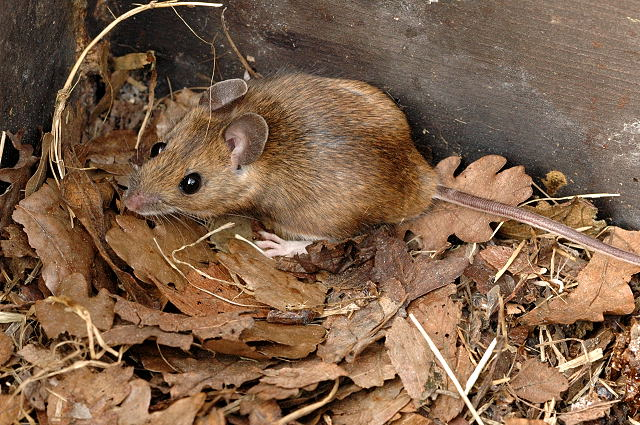
\includegraphics[width=0.3\textwidth]{mouse.jpg}
\caption{\label{fig:mice}yellow-necked mouse, from wikipedia.}
\end{figure}

This species lives mostly in woodlands and it is suspected that its distribution is limited by altitude. Let us compare a population living in the mountain (population $\boldsymbol{M}$) with a population living in the plain (population $\boldsymbol{P}$) to see if the altitude is a limiting distribution factor. This species can be described by a life-cylce in two stages; juveniles and adults. Thus the matrices describing those populations are given by:

\begin{equation}
\boldsymbol{P}=\begin{pmatrix}
0&2\\
0.25&0.5
\end{pmatrix}
\end{equation}
and
\begin{equation}
\boldsymbol{M}=\begin{pmatrix}
0&1.9\\
0.2&0.45
\end{pmatrix}
\end{equation}
Find the asymptotic growth rates of these populations. You can see that they differ. We would now like to investigate which matrix elements contribute the most to the difference in the asymptotic growth rates. For this we describe the asymptotic growth rate of the mountain population matrix, $\boldsymbol{M}$, as a function of the asymptotic growth rate of the plain population matrix, $\boldsymbol{P}$ , our reference population plus a treatment effect:  

\begin{equation}\label{a}
\lambda^{(M)} \approx \lambda^{(P)}+\sum_{i,j}{(a^{(M)}_{ij}-a^{(P)}_{ij})} \frac{ \partial\lambda^{A}}{\partial a^{A}_{ij}}
\end{equation}
Let us work through the right part of this equation together. 
\begin{itemize}
\item $\lambda^{(P)}$ is the asymptotic growth rate of the $\boldsymbol{P}$ matrix. 
\item The term ${(a^{(M)}_{ij}-a^{(P)}_{ij})}$, is the change in the elements of the matrix due to the treatment effect, here the moutain habitat. It tells us how different an element in matrix $\boldsymbol{M}$ is from the element at the same position in matrix $\boldsymbol{P}$.
\item The last part, $\frac{ \partial\lambda^{A}}{\partial a^{A}_{ij}}$, is the sensitivities of the asymptotic growth rate of a "mid-way" matrix to elements of that "mid-way" matrix. This matrix is the mean between $\boldsymbol{P}$ and $\boldsymbol{M}$ and is thus given by 
\begin{equation}
\boldsymbol{A}=\frac{\boldsymbol{M}+\boldsymbol{P}}{2}
\end{equation}
The matrix $\boldsymbol{A}$ is used because we need a matrix to compare matrices $\boldsymbol{P}$ and $\boldsymbol{M}$ against. It is possible to use either matrix $\boldsymbol{P}$ or $\boldsymbol{M}$ instead but this would give more weight to the selected matrix. Therefore we use the matrix that lies just in between.
\item The multiplication of the sensitivities with the summation term defines how much the change in each elements of the matrix due to the treatment affects the asymptotic growth rate. In other word they are the contributions of the $a_{ij}$ to the effect of the habitat on the growth. It is necessary to do this because for example, a large difference between the elements in the same position may in fact have little effect on the growth if the senstitivity for this position is low. 
\end{itemize}

You may have recognized that equation \ref{a} is a linear equation ($y=b+ax$). This method makes the assumption that the relationship between the matrices is linear and that the slope of this equation is given by $\frac{ \partial\lambda^{A}}{\partial a^{A}_{ij}}$.


With equation \ref{a}, find the value of $\lambda^{(\boldsymbol{M})}$ using \texttt{R} and compare it to the value you found earlier. How different are they? More interestingly: which difference in the matrix elements is mainly responsible for this difference? Is it the juvenile survival, the adult survival or the reproductive rate?\\[1.5ex]

\textit{Hint} Find the "mid-way" matrix. For the sensitivities, either approximate them yourself or use the \texttt{sensitivity()} function from the \texttt{popbio} package

\subsection{Fixed Factorial Designs (Theory)}
Factorial LTRE allows the examination of the effects of several treatments and their interactions. This is the case for your rotifer data where you have a "layer" treatment, a "pollution" treatment and a "species" treatment. Not all the combinations were investigated though; the layers "recovery" and "pollution" contained only the species BU whereas the layers "commercial" and "postpollution" contained only species BC. What difficulty would this pose if you want to compare the species to each other? Because of this, we cannot make a full factorial LTRE on the rotifer data, but we will examine subsets of the full dataset.


For example let us consider the species BU which has two treatments of the type "layer": the layers "recovery" ($r$) and "pollution" ($p$). For each of these layers it has 3 possible levels for the copper treatment: "low" ($l$), "medium" ($m$) and "high" ($h$). We thus have two factors, one with two levels, the second with three levels.

A factorial LTRE is similar to a one-way LTRE; we want to find which differences in matrix elements between a focal matrix and a reference matrix contribute the most to the difference in $\lambda$ between the two matrices. Let us take the matrix "recovery" and "low" which we call $\boldsymbol{M}^{r,l}$ as the focal matrix, for this we average the rates over all the $6$ replicates that were subject to this treatment ($r,l$). We compare it to the matrix naive to any treatment, which we call $\boldsymbol{M}^{..}$. This matrix is obtained from taking the average rates for all the matrices that we are comparing to each other (that is in this case the average of $\boldsymbol{M}^{r,l}$,$\boldsymbol{M}^{r,m}$,$\boldsymbol{M}^{r,h}$,$\boldsymbol{M}^{p,l}$,$\boldsymbol{M}^{p,m}$ and $\boldsymbol{M}^{p,h}$). Again we are interested in understanding the effect of the different treatments on the asymptotic growth rates.
\begin{equation}\label{b}
\lambda^{r,l}=\lambda^{..}+\alpha^{r}+\beta^{l}+(\alpha \beta)^{r,l}
\end{equation}
Equation \ref{b} tells us that $\lambda^{r,l}$ can be found from $\lambda^{..}$ plus an effect from the layer "recovery", an effect from the pollution "low" and an interaction between the two treatments.

To isolate the effect of each treatment, we need to look at them separately. So we examine a matrix $\boldsymbol{M}^{r.}$, where the effect of pollution is ignored. The rates of this matrix are calculated as the average of all the matrices with the layer "recovery". 
\begin{equation}\label{c}
\alpha^{r}=\sum_{ij}(a^{r.}_{ij}-a^{..}_{ij}) \frac{\partial\lambda^{A}}{\partial a^{A}_{ij}}
\end{equation}
The structure of equation \ref{c} is the same as the last part of equation \ref{a}. The matrix $\boldsymbol{A}$ is again a "mid-way" matrix between $\boldsymbol{M}^{r.}$ and $\boldsymbol{M}^{..}$. $\alpha^{r}$ tells us how large the effect of the treatment "layer" is on the asymptotic growth rate. If we want to know which matrix elements are responsible for this effect, we need to look at the separate contributions to $\alpha^r$ ($(a^{r.}_{ij}-a^{..}_{ij}) \frac{\partial\lambda^{A}}{\partial a^{A}_{ij}}$). Analogously we can also calculate $\alpha^p$.

We do the same for the second factor. We examine a matrix $\boldsymbol{M}^{.l}$, where the effect of the layer is ignored: 
\begin{equation}\label{d}
\beta^{l}=\sum_{ij}(a^{.l}_{ij}-a^{..}_{ij}) \frac{\partial\lambda^{B}}{\partial a^{B}_{ij}}
\end{equation}
For the interaction effect, we apply the same logic. We examine a matrix $\boldsymbol{M}^{rl}$ where both the effects of the layer and the pollution are taken into account so as to capture the effect of the interaction between the two factors. Because we want to isolate the interaction effect, we need to remove the effects of the layer and copper treatment.
\begin{equation}
(\alpha \beta)^{rl}=\sum_{ij}(a^{rl}_{ij}-a^{..}_{ij}) \frac{\partial\lambda^{C}}{\partial a^{C}_{ij}} -\alpha^{r}-\beta^{l}
\end{equation}
So far we have considered only the effect of the layer "recovery" and the pollution "low". Of course this can be extended to all other layers of all treatments. So in general the equations become for $k$ the level of treatment $1$ and $m$ the level of treatment $2$.

\begin{equation}\label{f}
\lambda^{k,m}=\lambda^{..}+\alpha^{k}+\beta^{m}+(\alpha \beta)^{k,m}
\end{equation}
\begin{equation}\label{e}
\alpha^{k}=\sum_{ij}(a^{k.}_{ij}-a^{..}_{ij}) \frac{\partial\lambda^{A}}{\partial a^{A}_{ij}}
\end{equation}
\begin{equation}
\beta^{m}=\sum_{ij}(a^{.m}_{ij}-a^{..}_{ij}) \frac{\partial\lambda^{B}}{\partial a^{B}_{ij}}
\end{equation}
\begin{equation}
(\alpha \beta)^{km}=\sum_{ij}(a^{km}_{ij}-a^{..}_{ij}) \frac{\partial\lambda^{C}}{\partial a^{C}_{ij}} -\alpha^{k}-\beta^{m}
\end{equation}
In these equations:
\begin{align}
A &= \frac{\boldsymbol{M^{k.}} + \boldsymbol{M^{..}}}{2} & B &= \frac{\boldsymbol{M^{.m}} + \boldsymbol{M^{..}}}{2} & C &= \frac{\boldsymbol{M^{km}} + \boldsymbol{M^{..}}}{2}
\end{align}
LTREs provide additional information to the growth rate as it describes how the different treatments affect the growth rate. In particular, LTRE allow a detailed comparison of the effect of a treatment on growth rate by examining the contribution of each survival and fertility rate to the gorwth rates of populations subjected to different treatment levels. For example, the graph below depicts the contribution of each element of populations under different copper levels to the growth rate. Each bar describes what is the contribution of an element to the growth rate when subjected to a given treatment level. What conclusions can you draw from this graph?





{\centering 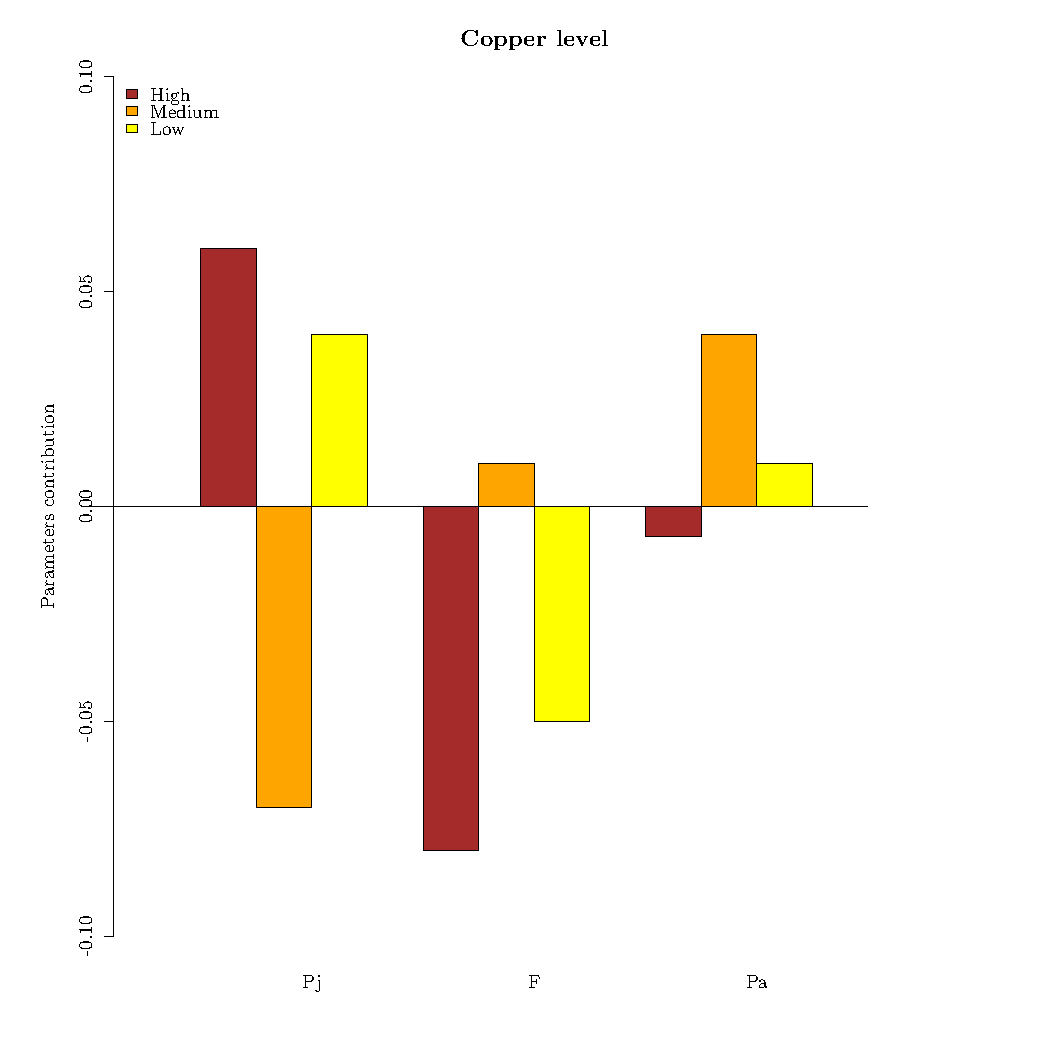
\includegraphics[width=\maxwidth]{figure/thypgraph-1} 

}




\section{Rotifer data analysis}
In this section, you will apply the factorial LTRE to the rotifer data to compare the layers "pollution" and "recovery". The second factor is the copper treatment with the levels "low", "high", "medium".
\begin{enumerate}
\item Load the file that contains the estimated transition rates in \texttt{R}, do not forget to set the working directory first. 
\item Because in the lab, you have made several replicates for each treatment combination, you now have a rate per replicate. We are however interested in the average rates per treatment. We want one juvenile survival rate, one adult survival rate and one fertility rate per population, per copper level and per species. For this you can use the \texttt{aggregate()} function that we have seen in practical $6$ and find the mean. Use the function three times seperately, once for each of the rates that we are interested in. Store the results in a variable. Use \texttt{?aggregate} to see how to use the function. You will need to use one special argument: \texttt{na.rm=TRUE}. This is to make sure that when there are $NA$s in the dataset, the function ignores them and still returns a value.
\item Now you have three separate lists. You want to group them. For this you can adapt the following lines of code. Use the names of the variables that you specified in the previous step.
\begin{knitrout}
\definecolor{shadecolor}{rgb}{0.969, 0.969, 0.969}\color{fgcolor}\begin{kframe}
\begin{alltt}
\hlstd{younewdata1}\hlkwb{<-}\hlkwd{merge}\hlstd{(SurvJuv, SurvAdu,} \hlkwc{by}\hlstd{=}\hlkwd{c}\hlstd{(}\hlnum{1}\hlstd{,}\hlnum{2}\hlstd{,}\hlnum{3}\hlstd{))}
\hlcom{#by set the column by which to merge the two elements}

\hlstd{younewdata2}\hlkwb{<-}\hlkwd{merge}\hlstd{(younewdata1, Fertility,} \hlkwc{by}\hlstd{=}\hlkwd{c}\hlstd{(}\hlnum{1}\hlstd{,}\hlnum{2}\hlstd{,}\hlnum{3}\hlstd{))}
\end{alltt}
\end{kframe}
\end{knitrout}
You can in addition give a more meaningful name to the columns by using:
\begin{knitrout}
\definecolor{shadecolor}{rgb}{0.969, 0.969, 0.969}\color{fgcolor}\begin{kframe}
\begin{alltt}
\hlkwd{colnames}\hlstd{(younewdata2)}\hlkwb{<-}\hlkwd{c}\hlstd{(}\hlstr{"name of col1"}\hlstd{,}
\hlstr{"name of col2"}\hlstd{,} \hlstr{"name of col3"}\hlstd{,}
\hlstr{"name of col4"}\hlstd{,} \hlstr{"name of col5"}\hlstd{,} \hlstr{"name of col6"}\hlstd{)}
\end{alltt}
\end{kframe}
\end{knitrout}
\item We mentioned that we are only interested at the moment in the layer "Recovery" and "Pollution". Both contained the species BU. Thus, select only the BU species with the \texttt{subset} function that we also used in practical $6$.
\item Below is a useful function for the LTRE. It allows you to extract a specific matrix per treatment by using \texttt{get\_matrix}. You need to give it the following arguments 1) the dataset from which you want to extract the matrix, 2) the name of the layer that you are interested in (for example "Pollution"), and 3) the name of the copper level (for example "high"). You do not need to understand the details of this code. If you run this code once during your \texttt{R}-session, \texttt{R} will remember it and every time you type \texttt{get\_matrix(data,layer,copper)} it will execute that code.
\begin{knitrout}
\definecolor{shadecolor}{rgb}{0.969, 0.969, 0.969}\color{fgcolor}\begin{kframe}
\begin{alltt}
\hlcom{#code for function to extract matrices from the dataset#}
\hlstd{get_matrix}\hlkwb{<-}\hlkwa{function}\hlstd{(}\hlkwc{roti}\hlstd{,}\hlkwc{pop}\hlstd{,}\hlkwc{cop}\hlstd{)\{}
  \hlkwa{if}\hlstd{(}\hlopt{!}\hlstd{pop} \hlopt \hlkwd{c}\hlstd{(}\hlkwd{levels}\hlstd{(roti}\hlopt{$}\hlstd{Population),}\hlstr{"mean"}\hlstd{))\{}
    \hlkwd{warning}\hlstd{(}\hlstr{"Something went wrong, give the instructors 
            a cookie and they may help you out:
            \textbackslash{}n------------------------\textbackslash{}n "}\hlstd{,pop,}
        \hlstr{" is not a valid entry\textbackslash{}n------------------------\textbackslash{}n"}\hlstd{)}

    \hlkwd{return}\hlstd{()}
  \hlstd{\}}

  \hlkwa{if}\hlstd{(}\hlopt{!}\hlstd{cop} \hlopt \hlkwd{c}\hlstd{(}\hlkwd{levels}\hlstd{(roti}\hlopt{$}\hlstd{Copper),}\hlstr{"mean"}\hlstd{))\{}
    \hlkwd{warning}\hlstd{(}\hlstr{"Something went wrong, give the instructors 
            a cookie and they may help you out:
            \textbackslash{}n------------------------\textbackslash{}n "}\hlstd{,cop,}\hlstr{" 
            is not a valid entry\textbackslash{}n------------------------\textbackslash{}n"}\hlstd{)}

    \hlkwd{return}\hlstd{()}
  \hlstd{\}}

  \hlkwa{if}\hlstd{(pop}\hlopt{==}\hlstr{"mean"} \hlopt{&} \hlstd{cop}\hlopt{==}\hlstr{"mean"}\hlstd{)\{}
    \hlstd{i}\hlkwb{<-}\hlnum{1}\hlopt{:}\hlkwd{length}\hlstd{(roti}\hlopt{$}\hlstd{Copper)}
  \hlstd{\}}\hlkwa{else if}\hlstd{(pop}\hlopt{==}\hlstr{"mean"}\hlstd{)\{}
    \hlstd{i}\hlkwb{<-}\hlkwd{which}\hlstd{(roti}\hlopt{$}\hlstd{Copper}\hlopt{==}\hlstd{cop)}
  \hlstd{\}}\hlkwa{else if}\hlstd{(cop}\hlopt{==}\hlstr{"mean"}\hlstd{)\{}
    \hlstd{i}\hlkwb{<-}\hlkwd{which}\hlstd{(roti}\hlopt{$}\hlstd{Population}\hlopt{==}\hlstd{pop)}
  \hlstd{\}}\hlkwa{else}\hlstd{\{}
    \hlstd{i}\hlkwb{<-}\hlkwd{which}\hlstd{(roti}\hlopt{$}\hlstd{Population}\hlopt{==}\hlstd{pop} \hlopt{&} \hlstd{roti}\hlopt{$}\hlstd{Copper}\hlopt{==}\hlstd{cop)}
  \hlstd{\}}

  \hlstd{A}\hlkwb{<-}\hlkwd{matrix}\hlstd{(}\hlkwd{c}\hlstd{(}\hlnum{0}\hlstd{,} \hlkwd{mean}\hlstd{(roti}\hlopt{$}\hlstd{Pj[i]),}
        \hlkwd{mean}\hlstd{(roti}\hlopt{$}\hlstd{F[i]),} \hlkwd{mean}\hlstd{(roti}\hlopt{$}\hlstd{Pa[i])),} \hlkwc{nrow}\hlstd{=}\hlnum{2}\hlstd{,} \hlkwc{ncol}\hlstd{=}\hlnum{2}\hlstd{)}
  \hlkwd{return}\hlstd{(A)}
  \hlstd{\}}
\hlcom{#end of the function#}
\end{alltt}
\end{kframe}
\end{knitrout}
\item With the \texttt{get\_matrix} function, extract the matrix for each treatment combinations ($6$ matrices in total). You need to specify the dataset in the first position, in the second position you need to specify the layer and in the third position the copper level.
\item Get the growth rate $\lambda$ of each of these matrix.
\item Now we get to the LTRE. Let us isolate the effect of the first treatment which is the layer. This factor has two levels; pollution and recovery. What we need to do is to implement equation \ref{e} in \texttt{R}. Let us find the $\alpha$ for the level "pollution" first; $\alpha^p$. 
\begin{enumerate}
\item Find the matrix $\boldsymbol{M}^{..}$. The rates of this matrix are the averages of the rates of all the matrices of the BU species. For this you can use the \texttt{get\_matrix} function.  The second argument concerns the layer, but here we want the mean rate over all the layers, we have written the function such that you can achieve this by typing "mean" as an argument for the layer. The same holds for the third argument.
\item Next you need the mean pollution matrix, $\boldsymbol{M}^{p.}$. Again, use the \texttt{get\_matrix} function.\\[1.5ex] 
\textit{small tip} Here you can do a little trick to be able to use the code later on a different subset of your dataset. Before using the \texttt{get\_matrix} function, set a new name to your focal layers like in the code below. Then in \texttt{get\_matrix}, instead of calling for "Pollution", call for \texttt{yourname1}.

\begin{knitrout}
\definecolor{shadecolor}{rgb}{0.969, 0.969, 0.969}\color{fgcolor}\begin{kframe}
\begin{alltt}
\hlstd{yourname1}\hlkwb{<-}\hlstr{'Pollution'}
\hlstd{yourname2}\hlkwb{<-}\hlstr{'Recovery'}
\end{alltt}
\end{kframe}
\end{knitrout}
\item Find the $\lambda$ for this matrix.
\item Find the "mid-way" matrix between $\boldsymbol{M}^{..}$ and $\boldsymbol{M}^{p.}$. This is the mean matrix between $\boldsymbol{M}^{..}$ and $\boldsymbol{M}^{p.}$.
\item For equation \ref{e}, you need the summation term and the sensitivity of the "mid-way" matrix. Let us look first at the summation term. You need the difference between the elements of matrix $\boldsymbol{M}^{p.}$ and of matrix $\boldsymbol{M}^{..}$. Thus take $(\boldsymbol{M}^{p.} - \boldsymbol{M}^{..})$. 
\item To find the sensitivity of the "mid-way" matrix, use the function \texttt{sensitivity} from the package \texttt{popbio} (see subsection \textit{sensitivity}). 
\item Finally, multiply the substraction matrix by the sensitivity matrix (not a matrix multiplication!) and save this in a matrix.
\item The sum of this matrix is your $\alpha^p$, the effect of the layer "Pollution" on the asymptotic growth rate. The separate entries of this matrix show how much each element of the population matrices contributes to the difference in $\lambda$ between them.
\item Store this matrix because the different elements of the matrix are what we are ultimately interested in. Check whether the effect you found indeed explains the difference between $\boldsymbol{M}^{..}$ and $\boldsymbol{M}^{p.}$.
\end{enumerate}
\item Repeat the same proceedure to find the second $\alpha$, $\alpha^r$ and store the separate contributions $(a^{k.}_{ij}-a^{..}_{ij}) \frac{\partial\lambda^{A}}{\partial a^{A}_{ij}}$. DO the same for the three values for $\beta$ and finally for the interactions. For the separate contribution of the interactions $(a^{km}_{ij}-a^{..}_{ij}) \frac{\partial\lambda^{C}}{\partial a^{C}_{ij}}$, do not forget to substract the corresponding contributions from the $\alpha$ and $\beta$. 
\item Once you have all the contributions of all the treatments, you may want to compare them. A possible graphs is a bar plot representing on the same graph the contribution to each parameter of each level of a factor, see for an example the graph above. If you agree that these sort of graphs are interesting, you can follow the next instructions. Feel free however to follow a different logic to produce the same graphs or to present your results in a different way. We do not claim to provide the most efficient code; any comments on how to improve the code are welcome.
\begin{enumerate}
\item Let us first look at the effect of the layer on the rates. One way of doing this is first to transform your matrices into vectors, using the \texttt{as.vector()} function and then combine the vector of each matrix into an array with \texttt{cbind()}. (you can actually ignore the first element of the matrices, the transition from juvenile to juvenile because it is always zero by selecting the vector elements 2 to 4). The columns are the layers and the row the rates. 
\item You can now use the \texttt{barplot()} command to plot bar graphs. Specify \texttt{beside=TRUE} to see the bars next to each other rather than on top of each other.
\item You may see that each bar (color) represents a rate although it would be more informative if each bar would be a layer. To correct for this, you can take the transpose of the array by using the function \texttt{t()} (we have seen this earlier this practical) and do the bar plot of the transpose. 
\item There are a few arguments you may want to use in the \texttt{barplot()} command to improve the visual appearance of the graph such as \texttt{xlab=}, \texttt{ylab=}, \texttt{xlim=c()}, \texttt{ylim=c()}, \texttt{col=c("colorname")}, \texttt{main="yourtitle"}.
\item Additionally, you may want to specify a legend and an axis. This you can do with the commands \texttt{legend()} and \texttt{axis()}. Look them up in the help section to see how to use them.
\item Don't forget to save your figures! A detailed description is given at the end of practical 6.
\end{enumerate}
\item Repeat all of the steps above for the combinations of the layers "Commercial" \& "Postpollution" and of the layers "Postpollution" \& "Pollution".
\end{enumerate}
If you manage to go through all the steps describe above, you should now know the growth rate of your populations, have performed three LTRE analyses on your rotifer data and have plots to include in your report. The interpretation of the results is up to you.


\begin{center}
Good luck!
\end{center}

\begin{figure}[h]
\centering
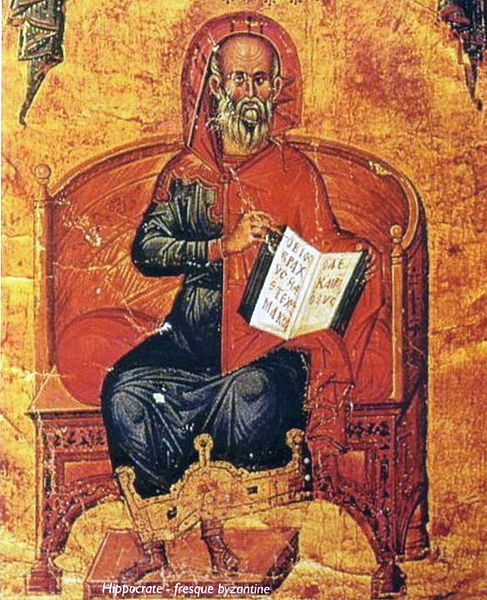
\includegraphics[width=0.3\textwidth]{Hippocrate.jpg}
\caption{\label{fig:owl}random picture, from wikipedia.}
\end{figure}



\begin{knitrout}
\definecolor{shadecolor}{rgb}{0.969, 0.969, 0.969}\color{fgcolor}\begin{kframe}
\begin{alltt}
\hlcom{#Open data}
\hlkwd{rm}\hlstd{(}\hlkwc{list} \hlstd{=} \hlkwd{ls}\hlstd{())}
\hlstd{rot}\hlkwb{<-}\hlkwd{read.csv}\hlstd{(}\hlstr{"BIO311_with_rates.csv"}\hlstd{,} \hlkwc{sep}\hlstd{=}\hlstr{","}\hlstd{)}
\hlkwd{str}\hlstd{(rot)}
\end{alltt}
\begin{verbatim}
## 'data.frame':	72 obs. of  13 variables:
##  $ Group.ID   : Factor w/ 6 levels "A","B","C","D",..: 1 1 1 1 1 1 1 1 1 1 ...
##  $ Population : Factor w/ 4 levels "Commercial","Pollution",..: 1 1 1 2 2 3 3 3 3 4 ...
##  $ Species    : Factor w/ 2 levels "BC","BU": 1 1 1 2 2 1 1 1 1 2 ...
##  $ Copper     : Factor w/ 3 levels "high","low","medium": 2 3 1 2 1 2 3 3 1 2 ...
##  $ Replicate  : int  1 6 4 2 3 6 2 4 2 1 ...
##  $ Day        : int  2 2 2 2 2 2 2 2 2 2 ...
##  $ Alive_Juv  : int  6 5 5 1 1 0 1 3 1 2 ...
##  $ Alive_Adult: int  7 8 7 5 3 2 3 4 2 6 ...
##  $ Dead_Juv   : int  0 0 0 0 0 0 0 1 0 0 ...
##  $ Dead_Adult : int  2 0 4 0 2 4 2 1 1 0 ...
##  $ Pj         : num  0.833 1 1 0 0 0 1 0 0 0.5 ...
##  $ Pa         : num  0.714 1 0.714 0 0.667 0 1 0.75 0.5 0.833 ...
##  $ F          : num  8 1.625 2 0 0.333 ...
\end{verbatim}
\begin{alltt}
\hlcom{#Find the avg rate per treatment}
\hlstd{Pj}\hlkwb{<-}\hlkwd{aggregate}\hlstd{(rot}\hlopt{$}\hlstd{Pj,} \hlkwd{list}\hlstd{(rot}\hlopt{$}\hlstd{Population, rot}\hlopt{$}\hlstd{Copper, rot}\hlopt{$}\hlstd{Species),}
              \hlkwc{na.rm}\hlstd{=}\hlnum{TRUE}\hlstd{,} \hlkwc{FUN}\hlstd{=}\hlstr{"mean"}\hlstd{)}
\hlstd{Pj}
\end{alltt}
\begin{verbatim}
##          Group.1 Group.2 Group.3         x
## 1     Commercial    high      BC 0.8916667
## 2  Postpollution    high      BC 0.4166667
## 3     Commercial     low      BC 0.8555000
## 4  Postpollution     low      BC 0.2500000
## 5     Commercial  medium      BC 0.9206667
## 6  Postpollution  medium      BC 0.4000000
## 7      Pollution    high      BU 0.5832500
## 8       Recovery    high      BU 0.7221667
## 9      Pollution     low      BU 0.5833333
## 10      Recovery     low      BU 0.5833333
## 11     Pollution  medium      BU 0.3195000
## 12      Recovery  medium      BU 0.2000000
\end{verbatim}
\begin{alltt}
\hlstd{Pa}\hlkwb{<-}\hlkwd{aggregate}\hlstd{(rot}\hlopt{$}\hlstd{Pa,} \hlkwd{list}\hlstd{(rot}\hlopt{$}\hlstd{Population, rot}\hlopt{$}\hlstd{Copper, rot}\hlopt{$}\hlstd{Species),}
              \hlkwc{na.rm}\hlstd{=}\hlnum{TRUE}\hlstd{,} \hlkwc{FUN}\hlstd{=}\hlstr{"mean"}\hlstd{)}
\hlstd{Pa}
\end{alltt}
\begin{verbatim}
##          Group.1 Group.2 Group.3         x
## 1     Commercial    high      BC 0.9523333
## 2  Postpollution    high      BC 0.5833333
## 3     Commercial     low      BC 0.9523333
## 4  Postpollution     low      BC 0.5832500
## 5     Commercial  medium      BC 0.9583333
## 6  Postpollution  medium      BC 0.5833333
## 7      Pollution    high      BU 0.8334000
## 8       Recovery    high      BU 0.9583333
## 9      Pollution     low      BU 0.6695000
## 10      Recovery     low      BU 0.8888333
## 11     Pollution  medium      BU 0.8790000
## 12      Recovery  medium      BU 0.7111667
\end{verbatim}
\begin{alltt}
\hlstd{F}\hlkwb{<-}\hlkwd{aggregate}\hlstd{(rot}\hlopt{$}\hlstd{F,} \hlkwd{list}\hlstd{(rot}\hlopt{$}\hlstd{Population, rot}\hlopt{$}\hlstd{Copper, rot}\hlopt{$}\hlstd{Species),}
             \hlkwc{na.rm}\hlstd{=}\hlnum{TRUE}\hlstd{,} \hlkwc{FUN}\hlstd{=}\hlstr{"mean"}\hlstd{)}
\hlstd{F}
\end{alltt}
\begin{verbatim}
##          Group.1 Group.2 Group.3         x
## 1     Commercial    high      BC 2.8556667
## 2  Postpollution    high      BC 0.5750000
## 3     Commercial     low      BC 3.3523333
## 4  Postpollution     low      BC 1.0000000
## 5     Commercial  medium      BC 2.2175000
## 6  Postpollution  medium      BC 1.1527778
## 7      Pollution    high      BU 0.5126000
## 8       Recovery    high      BU 0.5973333
## 9      Pollution     low      BU 0.8451667
## 10      Recovery     low      BU 0.8888333
## 11     Pollution  medium      BU 1.2013333
## 12      Recovery  medium      BU 0.5911667
\end{verbatim}
\begin{alltt}
\hlstd{Surv}\hlkwb{<-}\hlkwd{merge}\hlstd{(Pj, Pa,}  \hlkwc{by}\hlstd{=}\hlkwd{c}\hlstd{(}\hlnum{1}\hlstd{,}\hlnum{2}\hlstd{,}\hlnum{3}\hlstd{))}
\hlstd{Surv}
\end{alltt}
\begin{verbatim}
##          Group.1 Group.2 Group.3       x.x       x.y
## 1     Commercial    high      BC 0.8916667 0.9523333
## 2     Commercial     low      BC 0.8555000 0.9523333
## 3     Commercial  medium      BC 0.9206667 0.9583333
## 4      Pollution    high      BU 0.5832500 0.8334000
## 5      Pollution     low      BU 0.5833333 0.6695000
## 6      Pollution  medium      BU 0.3195000 0.8790000
## 7  Postpollution    high      BC 0.4166667 0.5833333
## 8  Postpollution     low      BC 0.2500000 0.5832500
## 9  Postpollution  medium      BC 0.4000000 0.5833333
## 10      Recovery    high      BU 0.7221667 0.9583333
## 11      Recovery     low      BU 0.5833333 0.8888333
## 12      Recovery  medium      BU 0.2000000 0.7111667
\end{verbatim}
\begin{alltt}
\hlcom{# Merge it into one dataset}
\hlstd{Roti}\hlkwb{<-}\hlkwd{merge}\hlstd{(Surv, F,} \hlkwc{by}\hlstd{=}\hlkwd{c}\hlstd{(}\hlnum{1}\hlstd{,}\hlnum{2}\hlstd{,}\hlnum{3}\hlstd{))}

\hlkwd{colnames}\hlstd{(Roti)}\hlkwb{<-} \hlkwd{c}\hlstd{(}\hlstr{"Population"}\hlstd{,} \hlstr{"Copper"}\hlstd{,} \hlstr{"Species"}\hlstd{,} \hlstr{"Pj"}\hlstd{,} \hlstr{"Pa"}\hlstd{,} \hlstr{"F"}\hlstd{)}
\hlstd{Roti}
\end{alltt}
\begin{verbatim}
##       Population Copper Species        Pj        Pa
## 1     Commercial   high      BC 0.8916667 0.9523333
## 2     Commercial    low      BC 0.8555000 0.9523333
## 3     Commercial medium      BC 0.9206667 0.9583333
## 4      Pollution   high      BU 0.5832500 0.8334000
## 5      Pollution    low      BU 0.5833333 0.6695000
## 6      Pollution medium      BU 0.3195000 0.8790000
## 7  Postpollution   high      BC 0.4166667 0.5833333
## 8  Postpollution    low      BC 0.2500000 0.5832500
## 9  Postpollution medium      BC 0.4000000 0.5833333
## 10      Recovery   high      BU 0.7221667 0.9583333
## 11      Recovery    low      BU 0.5833333 0.8888333
## 12      Recovery medium      BU 0.2000000 0.7111667
##            F
## 1  2.8556667
## 2  3.3523333
## 3  2.2175000
## 4  0.5126000
## 5  0.8451667
## 6  1.2013333
## 7  0.5750000
## 8  1.0000000
## 9  1.1527778
## 10 0.5973333
## 11 0.8888333
## 12 0.5911667
\end{verbatim}
\begin{alltt}
\hlcom{#Finding the lambda for each matrix (optional)}
\hlstd{Roti}\hlopt{$}\hlstd{lambda}\hlkwb{<-}\hlnum{NA}

\hlkwd{library}\hlstd{(}\hlstr{'popbio'}\hlstd{)}
\hlkwa{for} \hlstd{(i} \hlkwa{in} \hlnum{1}\hlopt{:}\hlkwd{length}\hlstd{(Roti}\hlopt{$}\hlstd{Pj))\{}
  \hlstd{M}\hlkwb{<-}\hlkwd{matrix}\hlstd{(}\hlkwd{c}\hlstd{(}\hlnum{0}\hlstd{, Roti}\hlopt{$}\hlstd{Pj[i], Roti}\hlopt{$}\hlstd{F[i], Roti}\hlopt{$}\hlstd{Pa[i]),} \hlkwc{nrow}\hlstd{=}\hlnum{2}\hlstd{,} \hlkwc{ncol}\hlstd{=}\hlnum{2}\hlstd{)}

  \hlstd{Roti}\hlopt{$}\hlstd{lambda[i]}\hlkwb{<-}\hlkwd{lambda}\hlstd{(M)}
\hlstd{\}}
 \hlstd{Roti}
\end{alltt}
\begin{verbatim}
##       Population Copper Species        Pj        Pa
## 1     Commercial   high      BC 0.8916667 0.9523333
## 2     Commercial    low      BC 0.8555000 0.9523333
## 3     Commercial medium      BC 0.9206667 0.9583333
## 4      Pollution   high      BU 0.5832500 0.8334000
## 5      Pollution    low      BU 0.5833333 0.6695000
## 6      Pollution medium      BU 0.3195000 0.8790000
## 7  Postpollution   high      BC 0.4166667 0.5833333
## 8  Postpollution    low      BC 0.2500000 0.5832500
## 9  Postpollution medium      BC 0.4000000 0.5833333
## 10      Recovery   high      BU 0.7221667 0.9583333
## 11      Recovery    low      BU 0.5833333 0.8888333
## 12      Recovery medium      BU 0.2000000 0.7111667
##            F    lambda
## 1  2.8556667 2.1414106
## 2  3.3523333 2.2353301
## 3  2.2175000 1.9862098
## 4  0.5126000 1.1041684
## 5  0.8451667 1.1126134
## 6  1.2013333 1.1990961
## 7  0.5750000 0.8614498
## 8  1.0000000 0.8704558
## 9  1.1527778 1.0307070
## 10 0.5973333 1.2921703
## 11 0.8888333 1.2905799
## 12 0.5911667 0.8502275
\end{verbatim}
\begin{alltt}
\hlcom{#----------- code for function to extract matrices from the dataset-----------#}
\hlstd{get_matrix}\hlkwb{<-}\hlkwa{function}\hlstd{(}\hlkwc{roti}\hlstd{,}\hlkwc{pop}\hlstd{,}\hlkwc{cop}\hlstd{)\{}
  \hlkwa{if}\hlstd{(}\hlopt{!}\hlstd{pop} \hlopt \hlkwd{c}\hlstd{(}\hlkwd{levels}\hlstd{(roti}\hlopt{$}\hlstd{Population),}\hlstr{"mean"}\hlstd{))\{}
    \hlkwd{warning}\hlstd{(}\hlstr{"Something went wrong, give the instructors a cookie and they may help you out:\textbackslash{}n------------------------\textbackslash{}n "}\hlstd{,}
            \hlstd{pop,}\hlstr{" is not a valid entry\textbackslash{}n------------------------\textbackslash{}n"}\hlstd{)}

    \hlkwd{return}\hlstd{()}
  \hlstd{\}}

  \hlkwa{if}\hlstd{(}\hlopt{!}\hlstd{cop} \hlopt \hlkwd{c}\hlstd{(}\hlkwd{levels}\hlstd{(roti}\hlopt{$}\hlstd{Copper),}\hlstr{"mean"}\hlstd{))\{}
    \hlkwd{warning}\hlstd{(}\hlstr{"Something went wrong, give the instructors a cookie and they may help you out:\textbackslash{}n------------------------\textbackslash{}n "}\hlstd{,}
            \hlstd{cop,}\hlstr{" is not a valid entry\textbackslash{}n------------------------\textbackslash{}n"}\hlstd{)}

    \hlkwd{return}\hlstd{()}
  \hlstd{\}}

  \hlkwa{if}\hlstd{(pop}\hlopt{==}\hlstr{"mean"} \hlopt{&} \hlstd{cop}\hlopt{==}\hlstr{"mean"}\hlstd{)\{}
    \hlstd{i}\hlkwb{<-}\hlnum{1}\hlopt{:}\hlkwd{length}\hlstd{(roti}\hlopt{$}\hlstd{Copper)}
  \hlstd{\}}\hlkwa{else if}\hlstd{(pop}\hlopt{==}\hlstr{"mean"}\hlstd{)\{}
    \hlstd{i}\hlkwb{<-}\hlkwd{which}\hlstd{(roti}\hlopt{$}\hlstd{Copper}\hlopt{==}\hlstd{cop)}
  \hlstd{\}}\hlkwa{else if}\hlstd{(cop}\hlopt{==}\hlstr{"mean"}\hlstd{)\{}
    \hlstd{i}\hlkwb{<-}\hlkwd{which}\hlstd{(roti}\hlopt{$}\hlstd{Population}\hlopt{==}\hlstd{pop)}
  \hlstd{\}}\hlkwa{else}\hlstd{\{}
    \hlstd{i}\hlkwb{<-}\hlkwd{which}\hlstd{(roti}\hlopt{$}\hlstd{Population}\hlopt{==}\hlstd{pop} \hlopt{&} \hlstd{roti}\hlopt{$}\hlstd{Copper}\hlopt{==}\hlstd{cop)}
  \hlstd{\}}

  \hlstd{A}\hlkwb{<-}\hlkwd{matrix}\hlstd{(}\hlkwd{c}\hlstd{(}\hlnum{0}\hlstd{,} \hlkwd{mean}\hlstd{(roti}\hlopt{$}\hlstd{Pj[i]),} \hlkwd{mean}\hlstd{(roti}\hlopt{$}\hlstd{F[i]),}
              \hlkwd{mean}\hlstd{(roti}\hlopt{$}\hlstd{Pa[i])),} \hlkwc{nrow}\hlstd{=}\hlnum{2}\hlstd{,} \hlkwc{ncol}\hlstd{=}\hlnum{2}\hlstd{)}
  \hlkwd{return}\hlstd{(A)}
  \hlstd{\}}
\hlcom{#--------------------------end of the function-----------------#}

\hlcom{#Get the matrices we are interested in (for Species BC)}
\hlkwd{library}\hlstd{(popbio)}
\hlstd{a}\hlkwb{<-}\hlstr{'Pollution'}
\hlstd{ash}\hlkwb{<-}\hlstr{'Poll'} \hlcom{# Short name for layer a}
\hlstd{b}\hlkwb{<-}\hlstr{'Recovery'}
\hlstd{bsh}\hlkwb{<-}\hlstr{'Rec'} \hlcom{# Short name for layer b}

\hlstd{Rotisub} \hlkwb{<-} \hlkwd{subset}\hlstd{(Roti, Roti}\hlopt{$}\hlstd{Population}\hlopt{==}\hlstd{a} \hlopt{|} \hlstd{Roti}\hlopt{$}\hlstd{Population}\hlopt{==}\hlstd{b)}
\hlstd{Rotisub}
\end{alltt}
\begin{verbatim}
##    Population Copper Species        Pj        Pa         F
## 4   Pollution   high      BU 0.5832500 0.8334000 0.5126000
## 5   Pollution    low      BU 0.5833333 0.6695000 0.8451667
## 6   Pollution medium      BU 0.3195000 0.8790000 1.2013333
## 10   Recovery   high      BU 0.7221667 0.9583333 0.5973333
## 11   Recovery    low      BU 0.5833333 0.8888333 0.8888333
## 12   Recovery medium      BU 0.2000000 0.7111667 0.5911667
##       lambda
## 4  1.1041684
## 5  1.1126134
## 6  1.1990961
## 10 1.2921703
## 11 1.2905799
## 12 0.8502275
\end{verbatim}
\begin{alltt}
\hlcom{#Here let us do the LTRE}
\hlcom{#two factors: population (1) and Copper (2)}
\hlcom{#The average matrix:}
\hlstd{M}\hlkwb{<-}\hlkwd{get_matrix}\hlstd{(Rotisub,} \hlstr{"mean"}\hlstd{,} \hlstr{"mean"}\hlstd{)}

\hlcom{#First the effect of population (1)-> alpha}
\hlstd{Pop1}\hlkwb{<-}\hlkwd{get_matrix}\hlstd{(Rotisub, a,} \hlstr{"mean"}\hlstd{)}
\hlcom{#Population level 3->Postpollution}
\hlcom{#Population level 1->Pollution }
     \hlcom{#Pollution}
       \hlcom{#The mid-way matrix }
\hlstd{A}\hlkwb{<-}\hlstd{((M}\hlopt{+}\hlstd{Pop1)}\hlopt{/}\hlnum{2}\hlstd{)}
\hlstd{alpha1}\hlkwb{<-}\hlstd{(Pop1}\hlopt{-}\hlstd{M)}\hlopt{*}\hlkwd{sensitivity}\hlstd{(A)}
\hlstd{alpha1}
\end{alltt}
\begin{verbatim}
##              [,1]        [,2]
## [1,]  0.000000000  0.02648626
## [2,] -0.001746024 -0.02259442
\end{verbatim}
\begin{alltt}
\hlcom{#Recovery}
\hlstd{Pop2}\hlkwb{<-}\hlkwd{get_matrix}\hlstd{(Rotisub, b,} \hlstr{"mean"}\hlstd{)}
       \hlcom{#The mid-way matrix }
\hlstd{B}\hlkwb{<-}\hlstd{((M}\hlopt{+}\hlstd{Pop2)}\hlopt{/}\hlnum{2}\hlstd{)}
\hlstd{alpha2}\hlkwb{<-}\hlstd{(Pop2}\hlopt{-}\hlstd{M)}\hlopt{*}\hlkwd{sensitivity}\hlstd{(B)}
\hlstd{alpha2}
\end{alltt}
\begin{verbatim}
##             [,1]        [,2]
## [1,] 0.000000000 -0.02727686
## [2,] 0.001610043  0.02307102
\end{verbatim}
\begin{alltt}
\hlcom{#Second the effect of Copper (2)-> beta}
\hlstd{hig}\hlkwb{<-}\hlkwd{get_matrix}\hlstd{(Rotisub,} \hlstr{"mean"}\hlstd{,} \hlstr{"high"}\hlstd{)}
\hlstd{med}\hlkwb{<-}\hlkwd{get_matrix}\hlstd{(Rotisub,} \hlstr{"mean"}\hlstd{,} \hlstr{"medium"}\hlstd{)}
\hlstd{low}\hlkwb{<-}\hlkwd{get_matrix}\hlstd{(Rotisub,} \hlstr{"mean"}\hlstd{,} \hlstr{"low"}\hlstd{)}
\hlcom{#Copper level 1->High}
\hlcom{#Copper leve 2->Medium}
\hlcom{#Copper leve 3->Low}
     \hlcom{#High}
       \hlcom{#The mid-way matrix }
\hlcom{#for beta:}
\hlstd{C}\hlkwb{<-}\hlstd{((M}\hlopt{+}\hlstd{hig)}\hlopt{/}\hlnum{2}\hlstd{)}
\hlstd{beta1}\hlkwb{<-}\hlstd{(hig}\hlopt{-}\hlstd{M)}\hlopt{*}\hlkwd{sensitivity}\hlstd{(C)}
\hlstd{beta1}
\end{alltt}
\begin{verbatim}
##            [,1]        [,2]
## [1,] 0.00000000 -0.08325026
## [2,] 0.06794042  0.05693927
\end{verbatim}
\begin{alltt}
  \hlcom{#Medium}
       \hlcom{#The mid-way matrix }
\hlcom{#for beta:}
\hlstd{D}\hlkwb{<-}\hlstd{((M}\hlopt{+}\hlstd{med)}\hlopt{/}\hlnum{2}\hlstd{)}

\hlstd{beta2}\hlkwb{<-}\hlstd{(med}\hlopt{-}\hlstd{M)}\hlopt{*}\hlkwd{sensitivity}\hlstd{(D)}
\hlstd{beta2}
\end{alltt}
\begin{verbatim}
##            [,1]        [,2]
## [1,]  0.0000000  0.03379360
## [2,] -0.1438248 -0.02240382
\end{verbatim}
\begin{alltt}
  \hlcom{#Low}
       \hlcom{#The mid-way matrix }
\hlcom{#for beta:}
\hlstd{E}\hlkwb{<-}\hlstd{((M}\hlopt{+}\hlstd{low)}\hlopt{/}\hlnum{2}\hlstd{)}

\hlstd{beta3}\hlkwb{<-}\hlstd{(low}\hlopt{-}\hlstd{M)}\hlopt{*}\hlkwd{sensitivity}\hlstd{(E)}
\hlstd{beta3}
\end{alltt}
\begin{verbatim}
##            [,1]        [,2]
## [1,] 0.00000000  0.03280523
## [2,] 0.04469452 -0.03349652
\end{verbatim}
\begin{alltt}
\hlcom{#Interactions}

\hlcom{#Here let us extract the 6 matrices we need:}
\hlstd{Pop1h}\hlkwb{<-}\hlkwd{get_matrix}\hlstd{(Rotisub, a,} \hlstr{"high"}\hlstd{)}
\hlstd{Pop1m}\hlkwb{<-}\hlkwd{get_matrix}\hlstd{(Rotisub, a,} \hlstr{"medium"}\hlstd{)}
\hlstd{Pop1l}\hlkwb{<-}\hlkwd{get_matrix}\hlstd{(Rotisub, a,} \hlstr{"low"}\hlstd{)}

\hlstd{Pop2h}\hlkwb{<-}\hlkwd{get_matrix}\hlstd{(Rotisub, b,} \hlstr{"high"}\hlstd{)}
\hlstd{Pop2m}\hlkwb{<-}\hlkwd{get_matrix}\hlstd{(Rotisub, b,} \hlstr{"medium"}\hlstd{)}
\hlstd{Pop2l}\hlkwb{<-}\hlkwd{get_matrix}\hlstd{(Rotisub, b,} \hlstr{"low"}\hlstd{)}

       \hlcom{#The mid-way matrix }
\hlcom{#for alpha:beta:}
\hlstd{F}\hlkwb{<-}\hlstd{((M}\hlopt{+}\hlstd{Pop1h)}\hlopt{/}\hlnum{2}\hlstd{)}

\hlstd{inter1}\hlkwb{<-}\hlstd{((Pop1h}\hlopt{-}\hlstd{M)}\hlopt{*}\hlkwd{sensitivity}\hlstd{(F))}\hlopt{-}\hlstd{alpha1}\hlopt{-}\hlstd{beta1}
\hlstd{inter1}
\end{alltt}
\begin{verbatim}
##            [,1]        [,2]
## [1,]  0.0000000 -0.04088048
## [2,] -0.0284428 -0.02644883
\end{verbatim}
\begin{alltt}
       \hlcom{#The mid-way matrix }
\hlcom{#for alpha:beta:}
\hlstd{G}\hlkwb{<-}\hlstd{((M}\hlopt{+}\hlstd{Pop1m)}\hlopt{/}\hlnum{2}\hlstd{)}
\hlcom{#The loop}

\hlstd{inter2}\hlkwb{<-}\hlstd{((Pop1m}\hlopt{-}\hlstd{M)}\hlopt{*}\hlkwd{sensitivity}\hlstd{(G))}\hlopt{-}\hlstd{alpha1}\hlopt{-}\hlstd{beta2}
\hlstd{inter2}
\end{alltt}
\begin{verbatim}
##            [,1]       [,2]
## [1,] 0.00000000 0.05434000
## [2,] 0.02999683 0.08829047
\end{verbatim}
\begin{alltt}
\hlcom{#The mid-way matrix }
\hlcom{#for alpha:beta:}
\hlstd{H}\hlkwb{<-}\hlstd{((M}\hlopt{+}\hlstd{Pop1l)}\hlopt{/}\hlnum{2}\hlstd{)}

\hlstd{inter3}\hlkwb{<-}\hlstd{((Pop1l}\hlopt{-}\hlstd{M)}\hlopt{*}\hlkwd{sensitivity}\hlstd{(H))}\hlopt{-}\hlstd{alpha1}\hlopt{-}\hlstd{beta3}
\hlstd{inter3}
\end{alltt}
\begin{verbatim}
##             [,1]        [,2]
## [1,] 0.000000000 -0.03349910
## [2,] 0.002175623 -0.05864936
\end{verbatim}
\begin{alltt}
\hlcom{#The mid-way matrix }
\hlcom{#for alpha:beta:}

\hlstd{I}\hlkwb{<-}\hlstd{((M}\hlopt{+}\hlstd{Pop2h)}\hlopt{/}\hlnum{2}\hlstd{)}
\hlstd{inter4}\hlkwb{<-}\hlstd{((Pop2h}\hlopt{-}\hlstd{M)}\hlopt{*}\hlkwd{sensitivity}\hlstd{(I))}\hlopt{-}\hlstd{alpha2}\hlopt{-}\hlstd{beta1}
\hlstd{inter4}
\end{alltt}
\begin{verbatim}
##            [,1]       [,2]
## [1,] 0.00000000 0.04235057
## [2,] 0.02797452 0.02575050
\end{verbatim}
\begin{alltt}
\hlcom{#The mid-way matrix }
\hlcom{#for alpha:beta:}
\hlstd{J}\hlkwb{<-}\hlstd{((M}\hlopt{+}\hlstd{Pop2m)}\hlopt{/}\hlnum{2}\hlstd{)}
\hlstd{inter5}\hlkwb{<-}\hlstd{((Pop2m}\hlopt{-}\hlstd{M)}\hlopt{*}\hlkwd{sensitivity}\hlstd{(J))}\hlopt{-}\hlstd{alpha2}\hlopt{-}\hlstd{beta2}
\hlstd{inter5}
\end{alltt}
\begin{verbatim}
##            [,1]        [,2]
## [1,]  0.0000000 -0.05759913
## [2,] -0.0217932 -0.09144026
\end{verbatim}
\begin{alltt}
\hlcom{#The mid-way matrix }
\hlcom{#for alpha:beta:}
\hlstd{K}\hlkwb{<-}\hlstd{((M}\hlopt{+}\hlstd{Pop2l)}\hlopt{/}\hlnum{2}\hlstd{)}
\hlstd{inter6}\hlkwb{<-}\hlstd{((Pop2l}\hlopt{-}\hlstd{M)}\hlopt{*}\hlkwd{sensitivity}\hlstd{(K))}\hlopt{-}\hlstd{alpha2}\hlopt{-}\hlstd{beta3}
\hlstd{inter6}
\end{alltt}
\begin{verbatim}
##              [,1]       [,2]
## [1,]  0.000000000 0.03395076
## [2,] -0.002051386 0.06077038
\end{verbatim}
\begin{alltt}
\hlcom{######### ARRANGING THE DATA FOR PLOTTING ##############}
\hlcom{#Copper}
\hlstd{Copper} \hlkwb{<-} \hlkwd{cbind}\hlstd{(}\hlkwd{as.vector}\hlstd{(beta1)[}\hlnum{2}\hlopt{:}\hlnum{4}\hlstd{],} \hlkwd{as.vector}\hlstd{(beta2)[}\hlnum{2}\hlopt{:}\hlnum{4}\hlstd{],}
                \hlkwd{as.vector}\hlstd{(beta3)[}\hlnum{2}\hlopt{:}\hlnum{4}\hlstd{])}
\hlkwd{colnames}\hlstd{(Copper)} \hlkwb{<-} \hlkwd{c}\hlstd{(}\hlstr{"High"}\hlstd{,} \hlstr{"Medium"}\hlstd{,} \hlstr{"Low"}\hlstd{)}
\hlkwd{rownames}\hlstd{(Copper)} \hlkwb{<-} \hlkwd{c}\hlstd{(}\hlstr{"Pj"}\hlstd{,} \hlstr{"F"}\hlstd{,} \hlstr{"Pa"}\hlstd{)}
\hlstd{Copper}
\end{alltt}
\begin{verbatim}
##           High      Medium         Low
## Pj  0.06794042 -0.14382485  0.04469452
## F  -0.08325026  0.03379360  0.03280523
## Pa  0.05693927 -0.02240382 -0.03349652
\end{verbatim}
\begin{alltt}
\hlstd{Coppert}\hlkwb{<-}\hlkwd{t}\hlstd{(Copper)}

\hlcom{#Layer}
\hlstd{Layer} \hlkwb{<-} \hlkwd{cbind}\hlstd{(}\hlkwd{as.vector}\hlstd{(alpha1)[}\hlnum{2}\hlopt{:}\hlnum{4}\hlstd{],} \hlkwd{as.vector}\hlstd{(alpha2)[}\hlnum{2}\hlopt{:}\hlnum{4}\hlstd{])}
\hlkwd{colnames}\hlstd{(Layer)} \hlkwb{<-} \hlkwd{c}\hlstd{(a, b)}
\hlkwd{rownames}\hlstd{(Layer)} \hlkwb{<-} \hlkwd{c}\hlstd{(}\hlstr{"Pj"}\hlstd{,} \hlstr{"F"}\hlstd{,} \hlstr{"Pa"}\hlstd{)}
\hlstd{Layer}
\end{alltt}
\begin{verbatim}
##       Pollution     Recovery
## Pj -0.001746024  0.001610043
## F   0.026486263 -0.027276861
## Pa -0.022594421  0.023071020
\end{verbatim}
\begin{alltt}
\hlstd{Layert}\hlkwb{<-}\hlkwd{t}\hlstd{(Layer)}

\hlcom{#Interactions}
\hlstd{Interactions} \hlkwb{<-} \hlkwd{cbind}\hlstd{(}\hlkwd{as.vector}\hlstd{(inter1)[}\hlnum{2}\hlopt{:}\hlnum{4}\hlstd{],} \hlkwd{as.vector}\hlstd{(inter2)[}\hlnum{2}\hlopt{:}\hlnum{4}\hlstd{],}
                      \hlkwd{as.vector}\hlstd{(inter3)[}\hlnum{2}\hlopt{:}\hlnum{4}\hlstd{],} \hlkwd{as.vector}\hlstd{(inter4)[}\hlnum{2}\hlopt{:}\hlnum{4}\hlstd{],}
                      \hlkwd{as.vector}\hlstd{(inter5)[}\hlnum{2}\hlopt{:}\hlnum{4}\hlstd{],} \hlkwd{as.vector}\hlstd{(inter6)[}\hlnum{2}\hlopt{:}\hlnum{4}\hlstd{])}
\hlkwd{colnames}\hlstd{(Interactions)} \hlkwb{<-} \hlstd{axislabels}
\end{alltt}


{\ttfamily\noindent\bfseries\color{errorcolor}{\#\# Error in eval(expr, envir, enclos): objet 'axislabels' introuvable}}\begin{alltt}
\hlkwd{rownames}\hlstd{(Interactions)} \hlkwb{<-} \hlkwd{c}\hlstd{(}\hlstr{"Pj"}\hlstd{,} \hlstr{"F"}\hlstd{,} \hlstr{"Pa"}\hlstd{)}
\hlstd{Interactions}
\end{alltt}
\begin{verbatim}
##           [,1]       [,2]         [,3]       [,4]
## Pj -0.02844280 0.02999683  0.002175623 0.02797452
## F  -0.04088048 0.05434000 -0.033499097 0.04235057
## Pa -0.02644883 0.08829047 -0.058649357 0.02575050
##           [,5]         [,6]
## Pj -0.02179320 -0.002051386
## F  -0.05759913  0.033950764
## Pa -0.09144026  0.060770385
\end{verbatim}
\begin{alltt}
\hlstd{Interactionst}\hlkwb{<-}\hlkwd{t}\hlstd{(Interactions)}

\hlcom{# Plotting}
\hlstd{ymin}\hlkwb{<-}\hlkwd{min}\hlstd{(}\hlkwd{c}\hlstd{(}\hlkwd{min}\hlstd{(Layer),}\hlkwd{min}\hlstd{(Copper),}\hlkwd{min}\hlstd{(Interactions)))}

\hlstd{ymax}\hlkwb{<-}\hlkwd{max}\hlstd{(}\hlkwd{c}\hlstd{(}\hlkwd{max}\hlstd{(Layer),}\hlkwd{max}\hlstd{(Copper),}\hlkwd{max}\hlstd{(Interactions)))}

\hlstd{ylim}\hlkwb{<-}\hlnum{0.03}\hlopt{+}\hlkwd{max}\hlstd{(}\hlkwd{c}\hlstd{(ymax,}\hlkwd{abs}\hlstd{(ymin)))}

\hlstd{limits}\hlkwb{<-}\hlkwd{c}\hlstd{(}\hlopt{-}\hlstd{ylim,ylim)}

\hlcom{#graphs}
\hlkwd{par}\hlstd{(}\hlkwc{mfrow}\hlstd{=}\hlkwd{c}\hlstd{(}\hlnum{1}\hlstd{,}\hlnum{3}\hlstd{),}\hlkwc{mar}\hlstd{=}\hlkwd{c}\hlstd{(}\hlnum{3}\hlstd{,}\hlnum{3}\hlstd{,}\hlnum{3}\hlstd{,}\hlnum{7}\hlstd{))}

\hlkwd{barplot}\hlstd{(Coppert,}\hlkwc{xaxt}\hlstd{=}\hlstr{'n'}\hlstd{,} \hlkwc{xlab}\hlstd{=}\hlstr{""}\hlstd{,} \hlkwc{ylab}\hlstd{=}\hlstr{"Parameters contribution"}\hlstd{,}
        \hlkwc{ylim}\hlstd{=limits,} \hlkwc{xlim}\hlstd{=}\hlkwd{c}\hlstd{(}\hlnum{0}\hlstd{,}\hlnum{14}\hlstd{),} \hlkwc{col}\hlstd{=}\hlkwd{c}\hlstd{(}\hlstr{"brown"}\hlstd{,}\hlstr{"orange"}\hlstd{,} \hlstr{"yellow"}\hlstd{),}
        \hlkwc{beside}\hlstd{=}\hlnum{TRUE}\hlstd{,} \hlkwc{main}\hlstd{=}\hlstr{"Copper level"}\hlstd{)}
\hlkwd{segments}\hlstd{(}\hlopt{-}\hlnum{1}\hlstd{,}\hlnum{0}\hlstd{,} \hlnum{13}\hlstd{,}\hlnum{0}\hlstd{)}
\hlkwd{par}\hlstd{(}\hlkwc{mar}\hlstd{=}\hlkwd{c}\hlstd{(}\hlnum{5.1}\hlstd{,} \hlnum{5.1}\hlstd{,} \hlnum{4.1}\hlstd{,} \hlnum{5.1}\hlstd{),} \hlkwc{xpd}\hlstd{=}\hlnum{TRUE}\hlstd{)}
\hlkwd{legend}\hlstd{(}\hlstr{"topleft"}\hlstd{,}
     \hlkwd{c}\hlstd{(}\hlstr{"High"}\hlstd{,} \hlstr{"Medium"}\hlstd{,} \hlstr{"Low"}\hlstd{),} \hlkwc{fill}\hlstd{=}\hlkwd{c}\hlstd{(}\hlstr{"brown"}\hlstd{,}\hlstr{"orange"}\hlstd{,} \hlstr{"yellow"}\hlstd{),}
     \hlkwc{bty}\hlstd{=}\hlstr{"n"}\hlstd{)}
\hlkwd{axis}\hlstd{(}\hlkwc{side}\hlstd{=}\hlnum{1}\hlstd{,} \hlkwc{at}\hlstd{=}\hlkwd{c}\hlstd{(}\hlnum{3}\hlstd{,}\hlnum{7}\hlstd{,}\hlnum{11}\hlstd{),} \hlkwc{labels}\hlstd{=}\hlkwd{c}\hlstd{(} \hlstr{"Pj"}\hlstd{,} \hlstr{"F"}\hlstd{,} \hlstr{"Pa"}\hlstd{),} \hlkwc{line}\hlstd{=}\hlnum{1}\hlstd{,}
     \hlkwc{tick}\hlstd{=}\hlnum{FALSE}\hlstd{)}

\hlkwd{barplot}\hlstd{(Layert,}\hlkwc{xaxt}\hlstd{=}\hlstr{'n'}\hlstd{,} \hlkwc{xlab}\hlstd{=}\hlstr{""}\hlstd{,} \hlkwc{ylab}\hlstd{=}\hlstr{""}\hlstd{,} \hlkwc{ylim}\hlstd{=limits,} \hlkwc{xlim}\hlstd{=}\hlkwd{c}\hlstd{(}\hlnum{0}\hlstd{,}\hlnum{14}\hlstd{),}
        \hlkwc{col}\hlstd{=}\hlkwd{c}\hlstd{(}\hlstr{"blue"}\hlstd{,}\hlstr{"lightblue"}\hlstd{),} \hlkwc{beside}\hlstd{=}\hlnum{TRUE}\hlstd{,} \hlkwc{main}\hlstd{=}\hlstr{"Layer"}\hlstd{)}
\hlkwd{segments}\hlstd{(}\hlopt{-}\hlnum{1}\hlstd{,}\hlnum{0}\hlstd{,} \hlnum{10}\hlstd{,}\hlnum{0}\hlstd{)}
\hlkwd{par}\hlstd{(}\hlkwc{mar}\hlstd{=}\hlkwd{c}\hlstd{(}\hlnum{5.1}\hlstd{,} \hlnum{5.1}\hlstd{,} \hlnum{4.1}\hlstd{,} \hlnum{5.1}\hlstd{),} \hlkwc{xpd}\hlstd{=}\hlnum{TRUE}\hlstd{)}
\hlkwd{legend}\hlstd{(}\hlstr{"topleft"}\hlstd{,}
     \hlkwd{c}\hlstd{(a,b),} \hlkwc{fill}\hlstd{=}\hlkwd{c}\hlstd{(}\hlstr{"blue"}\hlstd{,}\hlstr{"lightblue"}\hlstd{),} \hlkwc{bty}\hlstd{=}\hlstr{"n"}\hlstd{)}
\hlkwd{axis}\hlstd{(}\hlkwc{side}\hlstd{=}\hlnum{1}\hlstd{,} \hlkwc{at}\hlstd{=}\hlkwd{c}\hlstd{(}\hlnum{2}\hlstd{,}\hlnum{5}\hlstd{,}\hlnum{8}\hlstd{),} \hlkwc{labels}\hlstd{=}\hlkwd{c}\hlstd{(} \hlstr{"Pj"}\hlstd{,} \hlstr{"F"}\hlstd{,} \hlstr{"Pa"}\hlstd{),} \hlkwc{line}\hlstd{=}\hlnum{1}\hlstd{,} \hlkwc{tick}\hlstd{=}\hlnum{FALSE}\hlstd{)}



\hlcom{#Interaction}
\hlcom{#Layer}
\hlstd{axislabels}\hlkwb{<-}\hlkwd{c}\hlstd{()}
\hlkwa{for}\hlstd{(i} \hlkwa{in} \hlkwd{c}\hlstd{(ash,bsh))\{}
  \hlkwa{for}\hlstd{(j} \hlkwa{in} \hlkwd{c}\hlstd{(}\hlstr{"H"}\hlstd{,}\hlstr{"M"}\hlstd{,}\hlstr{"L"}\hlstd{))\{}
    \hlstd{axislabels}\hlkwb{<-}\hlkwd{c}\hlstd{(axislabels,}\hlkwd{paste}\hlstd{(i,j,}\hlkwc{sep}\hlstd{=}\hlstr{""}\hlstd{))}
  \hlstd{\}}
\hlstd{\}}

\hlstd{axislabels2}\hlkwb{<-}\hlkwd{c}\hlstd{()}
\hlkwa{for}\hlstd{(i} \hlkwa{in} \hlkwd{c}\hlstd{(ash,bsh))\{}
  \hlkwa{for}\hlstd{(j} \hlkwa{in} \hlkwd{c}\hlstd{(}\hlstr{"$+$"}\hlstd{,}\hlstr{"$\textbackslash{}\textbackslash{}pm$"}\hlstd{,}\hlstr{"$-$"}\hlstd{))\{}
    \hlstd{axislabels2}\hlkwb{<-}\hlkwd{c}\hlstd{(axislabels2,}\hlkwd{paste}\hlstd{(i,j,}\hlkwc{sep}\hlstd{=}\hlstr{"; "}\hlstd{))}
  \hlstd{\}}
\hlstd{\}}


\hlkwd{rainbow}\hlstd{(}\hlnum{6}\hlstd{,}\hlkwc{start} \hlstd{=} \hlnum{0}\hlstd{,} \hlkwc{end} \hlstd{=} \hlnum{0.5}\hlstd{,} \hlkwc{alpha} \hlstd{=} \hlnum{0.7}\hlstd{)}
\end{alltt}
\begin{verbatim}
## [1] "#FF0000B3" "#FF9900B3" "#CCFF00B3" "#33FF00B3"
## [5] "#00FF66B3" "#00FFFFB3"
\end{verbatim}
\begin{alltt}
\hlkwd{library}\hlstd{(}\hlstr{"RColorBrewer"}\hlstd{)}

\hlkwd{barplot}\hlstd{(Interactionst,} \hlkwc{xaxt}\hlstd{=}\hlstr{'n'}\hlstd{,} \hlkwc{xlab}\hlstd{=}\hlstr{""}\hlstd{,} \hlkwc{ylab}\hlstd{=}\hlstr{""}\hlstd{,} \hlkwc{ylim}\hlstd{=limits,} \hlkwc{xlim}\hlstd{=}\hlkwd{c}\hlstd{(}\hlnum{0}\hlstd{,}\hlnum{20}\hlstd{),}
        \hlkwc{col}\hlstd{=}\hlkwd{brewer.pal}\hlstd{(}\hlnum{6}\hlstd{,} \hlstr{"Set3"}\hlstd{) ,} \hlkwc{beside}\hlstd{=}\hlnum{TRUE}\hlstd{,} \hlkwc{main}\hlstd{=}\hlstr{"Interactions"}\hlstd{)}
\hlkwd{segments}\hlstd{(}\hlopt{-}\hlnum{1}\hlstd{,}\hlnum{0}\hlstd{,} \hlnum{20}\hlstd{,}\hlnum{0}\hlstd{)}
\hlkwd{par}\hlstd{(}\hlkwc{mar}\hlstd{=}\hlkwd{c}\hlstd{(}\hlnum{5.1}\hlstd{,} \hlnum{5.1}\hlstd{,} \hlnum{4.1}\hlstd{,} \hlnum{7.1}\hlstd{),} \hlkwc{xpd}\hlstd{=}\hlnum{TRUE}\hlstd{)}
\hlkwd{legend}\hlstd{(}\hlstr{"topleft"}\hlstd{,}
     \hlstd{axislabels2,} \hlkwc{fill}\hlstd{=}\hlkwd{brewer.pal}\hlstd{(}\hlnum{6}\hlstd{,} \hlstr{"Set3"}\hlstd{),} \hlkwc{bty}\hlstd{=}\hlstr{"n"}\hlstd{,} \hlkwc{ncol}\hlstd{=}\hlnum{2}\hlstd{,}\hlkwc{text.width}\hlstd{=}\hlnum{5}\hlstd{)}
\hlkwd{axis}\hlstd{(}\hlkwc{side}\hlstd{=}\hlnum{1}\hlstd{,} \hlkwc{at}\hlstd{=}\hlkwd{c}\hlstd{(}\hlnum{5}\hlstd{,}\hlnum{12}\hlstd{,}\hlnum{18}\hlstd{),} \hlkwc{labels}\hlstd{=}\hlkwd{c}\hlstd{(} \hlstr{"Pj"}\hlstd{,} \hlstr{"F"}\hlstd{,} \hlstr{"Pa"}\hlstd{),} \hlkwc{line}\hlstd{=}\hlnum{1}\hlstd{,} \hlkwc{tick}\hlstd{=}\hlnum{FALSE}\hlstd{)}
\end{alltt}
\end{kframe}
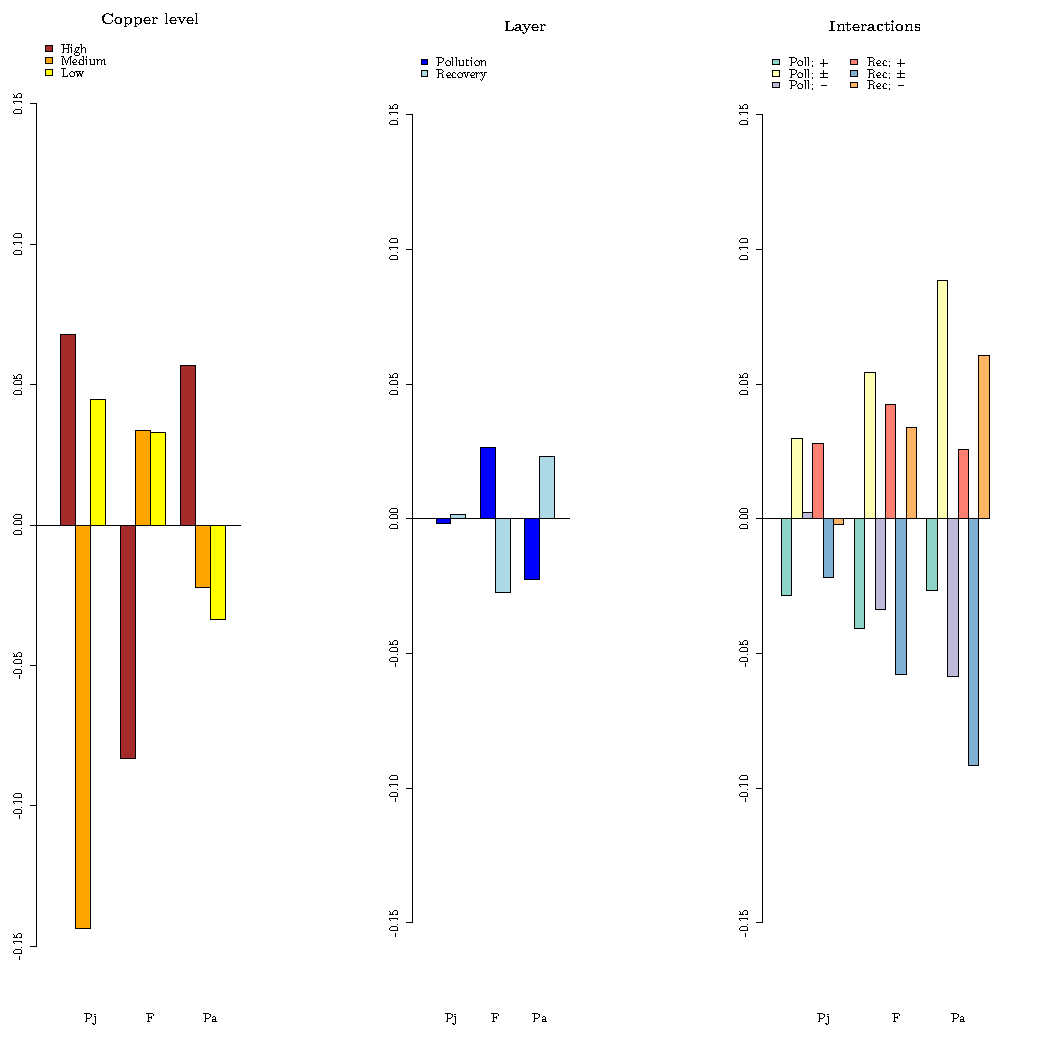
\includegraphics[width=\maxwidth]{figure/tReco_vs_Post-1} 

\end{knitrout}


\end{document}
